\documentclass{standalone}

\usepackage[american]{circuitikz}

\begin{document}
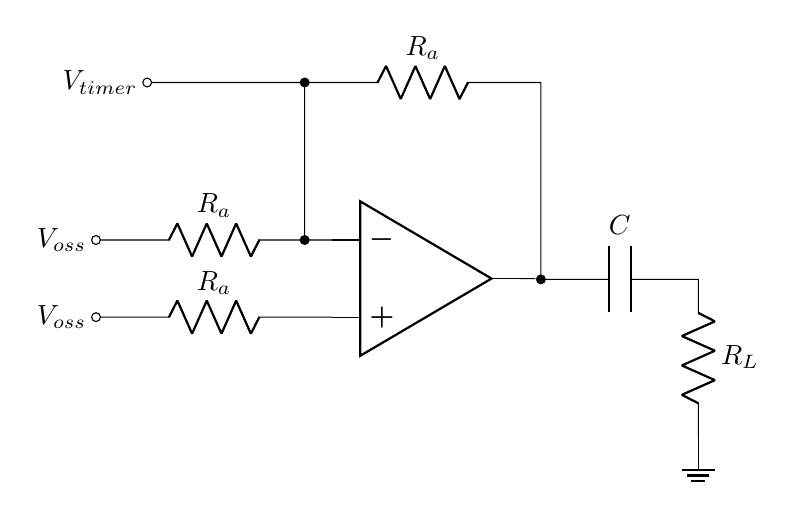
\begin{tikzpicture}
	\draw
	(0,0) node[op amp] (opamp) {}
	(opamp.+) to [R, l_=$R_a$, -o] ++(-3,0) node[left] {$V_{oss}$}
	(opamp.-) to [R, l_=$R_a$, -o] ++(-3,0) node[left] {$V_{oss}$}
	(opamp.-) to [short] ++(-0.35,0) to [short, *-*] ++(0, 2) coordinate(point1)
	(point1) to [short, -o] ++(-2,0) node[left] {$V_{timer}$}
	(point1) to [R, l=$R_a$] ++(3, 0)
	to [short, -*] ++(0, -2.5)
	to [C, l=$C$] ++(2,0)
	to [R, l=$R_L$] ++(0,-2) node[ground] {}
	(opamp.out) to[short] ++(0.2, 0)
	;
\end{tikzpicture}
\end{document}